\documentclass[border=5pt]{standalone}
\usepackage[utf8]{inputenc}
\usepackage{amssymb}
\usepackage{amsmath}
\usepackage{tikz}
\usetikzlibrary{arrows.meta}

\begin{document}
\nopagecolor
\begin{tabular}{c}
    Directed minimum sampled spanning tree $\vec{T}^*$ \\ \\
    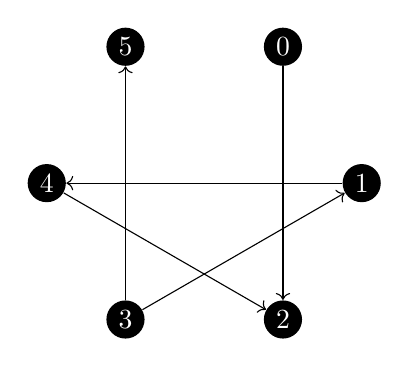
\begin{tikzpicture}
        \node[circle, inner sep=2pt, fill] (0) at (1, 1.732) {\color{white} 0};
        \node[circle, inner sep=2pt, fill] (1) at (2, 0) {\color{white} 1};
        \node[circle, inner sep=2pt, fill] (2) at (1, -1.732) {\color{white} 2};
        \node[circle, inner sep=2pt, fill] (3) at (-1, -1.732) {\color{white} 3};
        \node[circle, inner sep=2pt, fill] (4) at (-2, 0) {\color{white} 4};
        \node[circle, inner sep=2pt, fill] (5) at (-1, 1.732) {\color{white} 5};

        \draw (0) edge[->] (2)
              (1) edge[->] (4)
              (3) edge[->] (1)
              (3) edge[->] (5)
              (4) edge[->] (2);
    \end{tikzpicture} \\ \\
    Minimum flow in the graph \\ \\
    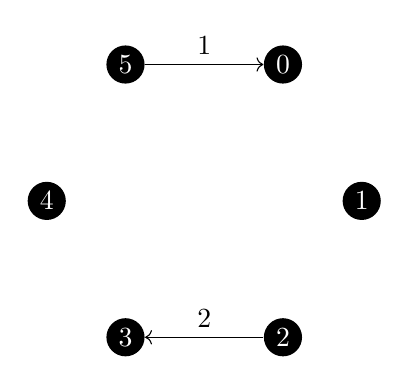
\begin{tikzpicture}
        \node[circle, inner sep=2pt, fill] (0) at (1, 1.732) {\color{white} 0};
        \node[circle, inner sep=2pt, fill] (1) at (2, 0) {\color{white} 1};
        \node[circle, inner sep=2pt, fill] (2) at (1, -1.732) {\color{white} 2};
        \node[circle, inner sep=2pt, fill] (3) at (-1, -1.732) {\color{white} 3};
        \node[circle, inner sep=2pt, fill] (4) at (-2, 0) {\color{white} 4};
        \node[circle, inner sep=2pt, fill] (5) at (-1, 1.732) {\color{white} 5};

        \draw (5) edge[->] node[above]{1} (0)
              (2) edge[->] node[above]{2} (3);
    \end{tikzpicture} \\ \\
    Incorrect circulation \\ \\
    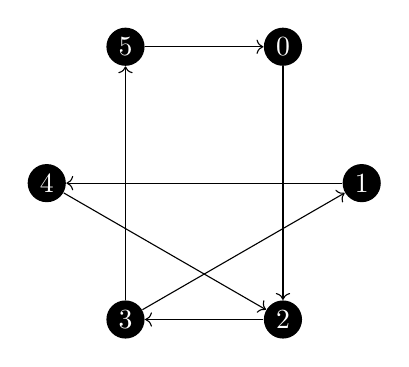
\begin{tikzpicture}
        \node[circle, inner sep=2pt, fill] (0) at (1, 1.732) {\color{white} 0};
        \node[circle, inner sep=2pt, fill] (1) at (2, 0) {\color{white} 1};
        \node[circle, inner sep=2pt, fill] (2) at (1, -1.732) {\color{white} 2};
        \node[circle, inner sep=2pt, fill] (3) at (-1, -1.732) {\color{white} 3};
        \node[circle, inner sep=2pt, fill] (4) at (-2, 0) {\color{white} 4};
        \node[circle, inner sep=2pt, fill] (5) at (-1, 1.732) {\color{white} 5};

        \draw (0) edge[->] (2)
              (1) edge[->] (4)
              (2) edge[->] (3)
              (3) edge[->] (1)
              (3) edge[->] (5)
              (4) edge[->] (2)
              (5) edge[->] (0);
    \end{tikzpicture} \\ \\
    Correct circulation \\ \\
    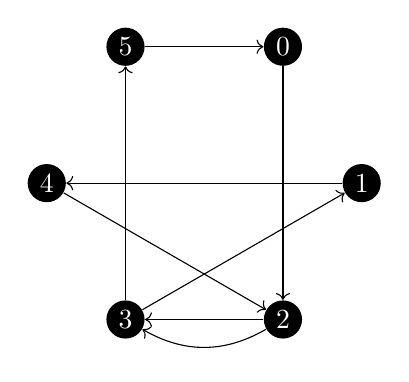
\begin{tikzpicture}
        \node[circle, inner sep=2pt, fill] (0) at (1, 1.732) {\color{white} 0};
        \node[circle, inner sep=2pt, fill] (1) at (2, 0) {\color{white} 1};
        \node[circle, inner sep=2pt, fill] (2) at (1, -1.732) {\color{white} 2};
        \node[circle, inner sep=2pt, fill] (3) at (-1, -1.732) {\color{white} 3};
        \node[circle, inner sep=2pt, fill] (4) at (-2, 0) {\color{white} 4};
        \node[circle, inner sep=2pt, fill] (5) at (-1, 1.732) {\color{white} 5};

        \draw (0) edge[->] (2)
              (1) edge[->] (4)
              (2) edge[->, bend left] (3)
              (2) edge[->] (3)
              (3) edge[->] (1)
              (3) edge[->] (5)
              (4) edge[->] (2)
              (5) edge[->] (0);
    \end{tikzpicture}
\end{tabular}
\end{document}